% !TEX encoding = UTF-8 Unicode


\chapter{Construção de espaços de probabilidade básicos}

Nessa seção descreveremos diversas maneiras diferentes de construir um espaço de probabilidade, dando diversos exemplos
de como elas podem ser usadas na modelagem de diferentes processos reais.

\section{Caso enumerável}

Quando $\Omega$ é finito ou enumerável, tipicamente definimos sobre $\Omega$ a $\sigma$-álgebra das partes, ou seja $\mathcal{F} = \mathcal{P}(\Omega) = \sigma(\{\omega\}_{\omega \in \Omega})$.
Além disso podemos definir probabilidades sobre $(\Omega, \mathcal{F})$ de maneira simples tomando $(p_\omega)_{\omega \in \Omega}$ tais que
\begin{enumerate}[\quad a)]
\item $p_\omega \geq 0$ para todo $\omega \in \Omega$ e
\item $\sum_{\omega \in \Omega} p_\omega = 1$.
\end{enumerate}
De fato, nesse caso definimos $P(A) = \sum_{\omega \in A} p_\omega$ que claramente define uma probabilidade.

\begin{exercise}
  Mostre que se $\Omega$ é finito ou enumerável, toda probabilidade sobre $(\Omega, \mathcal{P}(\Omega))$ é dada como na descrição acima.
\end{exercise}

\begin{example} \mbox{}
  \begin{enumerate}[\quad a)]
  \item Lembramos do Exemplo~\ref{x:bernoulli} a distribuição de Bernoulli.
  \item Dados $n \geq 1$ e $p \in [0,1]$, definimos a medida $\Bin(n,p)$ \index{distribuicao@distribuição!binomial} (binomial) em $\Omega = \{0, 1, \dots, n\}$ com
    \begin{equation}
      p_i = \binom ni p^i (1-p)^{n-i}, \text{ para $i \in \Omega$.}
    \end{equation}
  \item Dado $p \in (0,1]$, em $\Omega = \{0, 1, \dots\}$ definimos a medida $\Geo(p)$ \index{distribuicao@distribuição!geometrica@geométrica} (geométrica) em $\Omega$ induzida pelos pesos
  \begin{equation}
    p_i = (1-p)^i p, \text{ para $i \geq 1$.}
  \end{equation}
  \end{enumerate}
\end{example}

\begin{exercise}
  Seja $\Omega = \{0,1\}^n$ e $p_\omega = \tfrac 1{2^n}$ para todo $\omega \in \Omega$ (ou seja a probabilidade uniforme).
  Considere $X: \Omega \to \{0,1, \dots, n\}$ dada por $X(\omega_1, \dots, \omega_n) = \sum_{i=1}^n \omega_i$.
  Obtenha a distribuição $P_X$.
  Dê um exemplo de medida em $\omega$ para a qual a distribuição de $X$ seja $\Bin(n,p)$.
\end{exercise}

\begin{topics}

\section{Tópico: Método Probabilístico}

Uma importante ferramenta em várias áreas da matemática, tais como Teoria dos Números, Combinatória e Teoria da Computação é o que chamamos de Método Probabilístico. \index{Metodo Probabilistico@Método Probabilístico}

Em várias situações, nós precisamos de mostrar a existência de objetos satisfazendo determinadas propriedades, mas não temos informação suficiente ou capacidade para construí-los explicitamente.
Nesse caso, podemos recorrer ao Método Probabilístico, que simplesmente nos sugere tomar um objeto aleatório de uma maneira esperta e mostrar que com probabilidade positiva as propriedades desejadas serão satisfeitas.
Esse método, apesar de muito ingênuo, é muito eficiente e em diversos casos provê os melhores exemplos conhecidos de certos objetos (para embaraço da comunidade científica).

Nessa seção daremos um exemplo em Teoria dos Números provido primeiramente por Erdõs\footnote{Somos gratos a Robert Morris por sugerir esse teorema como exemplo do Método Probabilístico.}.

\begin{theorem}[Erdös]
  Para todo conjunto finito $A \subset \mathbb{N}$, existe um sub-conjunto $B \subseteq A$ satisfazendo
  \begin{enumerate}[\quad a)]
  \item $\# B \geq \frac{\#A}{3}$ e tal que
  \item não existem $x, y$ e $z \in B$ com $x + y = z$.
  \end{enumerate}
  A propriedade $b)$ acima é o que chamamos de um conjunto ser livre de somas. \index{conjunto!livre de somas}
\end{theorem}

Certamente não temos muita informação sobre $A$, então vamos usar o método probabilístico para a prova desse teorema.

\begin{proof}
  Fixamos $p$ um número primo maior que três vezes o maior elemento de $A$ e considere o espaço $\mathbb{Z}_p$ dos inteiros módulo $p$.
  Seja $X$ um elemento aleatório de $\mathbb{Z}_p$ com distribuição uniforma, isto é $U_{\{0, \dots, p-1\}}$.
  \begin{exercise}
    Mostre que para todo $a \in A$, a multiplicação por $a$ é uma bijeção em $\mathbb{Z}_p$, ou seja
    \begin{equation}
      \mathbb{Z}_p \cdot a = \mathbb{Z}_p.
    \end{equation}
    onde o produto $\mathbb{Z}_p \cdot a$ é entendido elemento a elemento.
    Conclua que
    \begin{equation}
      P \Big[ X \cdot a \in \big[ \tfrac{p}{3}, \tfrac {2p}{3} \big) \Big] \geq \frac{1}{3} -\frac{1}{p}.
    \end{equation}
  \end{exercise}
  Definimos o conjunto aleatório
  \begin{equation}
    \mathcal{B} = \{ x \in A \ | X \cdot a \in [\tfrac p3, \tfrac {2p}3) \}.
  \end{equation}
  Esse conjunto é livre de soma: se $X=0$, o conjunto é vazio e, nos outros casos, se $x, y \in \mathcal{B}$ então
  \begin{equation}
    X (x+y)\in [\tfrac {2p}3, \tfrac {4p} 3)
  \end{equation}
  que é o complemento de $[\tfrac{p}{3}, \tfrac{2p}{3} )$ em $\mathbb{Z}_p$.
  \medskip

  Basta portanto mostrar que com probabilidade positiva $\# \mathcal{B} \geq \tfrac{\#A}3$, que segue do seguinte argumento.
  Note inicialmente que
  \begin{multline*}
    \int \# \mathcal{B} \d P = \int \sum_{a \in A} \1_{\big[ X \cdot a \in [p/3, 2p/3) \big]} \d P \\
    =
    \sum_{a \in A} P \Big[ X \cdot a \in \big[ \tfrac{p}{3}, \tfrac {2p}{3} \big) \Big] \geq \frac{\# A}{3}- \frac{\# A}{p}> \frac{\# A-1 }{3},
  \end{multline*}
  mas, para qualquer variável aleatória,  $P[Y \geq \int Y \d P] > 0$.
  Nesse caso, isso implica
    \begin{equation}
      P[ \# \mathcal{B} \ge \tfrac{\# A}3 ] =  P[ \# \mathcal{B} > \tfrac{\# A-1 }3 ] \geq P \Big[ \# \mathcal{B} > \int \# \mathcal{B} \d P \Big] >0.
    \end{equation}
\end{proof}

\todo{Adicionar contexto histórico: citar artigo Erdos e o Annals of Math que mostra que não é possível com $\#A(1/3 + \varepsilon)$.}

\end{topics}

\vfill
\pagebreak

\section{Caso absolutamente contínuo}

Uma outra maneira simples de definir um espaço de probabilidade é partindo de um espaço de medida.
Seja $(\Omega, \mathcal{F}, \mu)$ um espaço de medida e $\rho:\Omega \to \mathbb{R}_+$ uma função mensurável com $\int \rho(x) \mu(\d x) = 1$.
Então podemos definir a probabilidade induzida
\begin{equation}
  \label{e:absolutamente_cont}
  P(A) = \int_A \rho(x) \mu(\d x).
\end{equation}
Nesse caso, chamamos $\rho$ de a \emph{densidade} \index{densidade} de $P$ com respeito a $\mu$.
Uma outra possível notação para a equação acima é $\d P = \rho(x) \d \mu$ \index{dP@$\d P = \rho \d \mu$} (lembrando a derivada de Radon-Nikodym).

Observe que o caso discreto pode ser definido em termos de uma densidade, onde $\rho(\omega) = p_\omega$ e $\mu$ é a medida da contagem em $\Omega$.

\begin{example}
  Vários exemplos podem ser obtidos via \eqref{e:absolutamente_cont} se tomamos $\Omega \subseteq \mathbb{R}$ e $\mu$ a medida de Lebesgue restrita a $\Omega$.
  Nesses casos, escrevemos $P = \rho(x) \d x$ em $\Omega$.
  Alguns exemplos importantes são:
  \begin{enumerate}[\quad a)]
  \item Para $a < b \in \mathbb{R}$, definimos a medida $U[a,b]$ \index{distribuicao@distribuição!uniforme} usando $\rho(x) = \tfrac{1}{b-a}\1_{[a,b]}(x)$.
  \item Para $\lambda > 0$, definimos a medida $\Exp(\lambda)$ \index{distribuicao@distribuição!exponencial} (chamada exponencial de parâmetro $\lambda$) por meio da densidade $\rho(x) = \lambda \exp\{-\lambda x\}$ em $[0,\infty)$.
  \end{enumerate}
\end{example}

Podemos também usar a distribuição de um elemento aleatório para construir outras probabilidades, como mostra o seguinte exemplo.

\begin{example}
  Considere por exemplo $X:[0,2\pi] \to \mathbb{C}$ dada por $X(t) = \exp\{-i t\}$.
  A distribuição imagem $X_*U_{[0,2\pi]}$ é o que chamamos de distribuição uniforme em $\bbS^1$, também denotada por $U_{S^1}$.
\end{example}

\begin{exercise}
  Mostre que $U_{\bbS^1}$ não é absolutamente contínua com respeito à medida de Lebesgue em $\mathbb{C} \sim \mathbb{R}^2$.
\end{exercise}

\begin{exercise}
  Mostre que $U_{\bbS^1}$ é invariante por rotações rígidas de $\mathbb{C}$, isto é, se $T:\mathbb{C} \to \mathbb{C}$ é uma isometria linear,
  $T_*U_{\bbS^1}=U_{\bbS^1}$.
\end{exercise}

\begin{exercise}
  Construa uma probabilidade em $S^2$ invariante por rotações.
\end{exercise}

\section{Um caso importante: $\gO=\bbR$}

\subsection{Funções acumuladas de distribuição}

Um caso muito importante de espaço amostral é $\Omega = \mathbb{R}$, principalmente por nos ajudar a entender distribuições de variáveis aleatórias.
Para tanto, precisaremos de uma boa ferramenta para descrever probabilidades em $\mathbb{R}$.

\begin{definition}
  Dada $P$ em $\mathbb{R}$, definimos $F_P:\mathbb{R} \to [0,1]$ por $F_P(x) = P\big((-\infty, x]\big)$.
  Essa função é chamada a \emph{função de distribuição} acumulada de $P$. \index{funcao de distribuicao@função de distribuição}
\end{definition}

\begin{notation}
  Se $X:\Omega \to \mathbb{R}$ é uma variável aleatória num espaço $(\Omega, \mathcal{F}, P)$, denotamos por $F_X$ \index{FX@$F_X$}
  a função de distribuição acumulada correspondente à distribuição $X_*P$.
\end{notation}

Lembramos que uma probabilidade em $\mathbb{R}$ é uma função $P:\mathcal{B}(\mathbb{R}) \to [0,1]$ e o domínio dessa função é bastante complicado.
Por exemplo se quisermos representar uma distribuição de uma variável aleatória no computador através dessa função $P$, teríamos problemas.
Contudo, a função $F_P$ (ou $F_X$) é muito mais simples de ser compreendida ou representada, por seu domínio ser $\mathbb{R}$.

\begin{example}
  Não é difícil verificar que
  \begin{equation}
    F_{\delta_{x_0}} =
    \begin{cases}
      0 & \text{ se $x < x_0$,}\\
      1 & \text{ se $x \geq x_0$}
    \end{cases}
  \end{equation}
  e que
  \begin{equation}
    F_{U_{[0,1]}} =
    \begin{cases}
      0 & \text{ se $x \leq 0$,}\\
      x & \text{ se $x \in [0,1]$ e}\\
      1 & \text{ se $x \geq 1$.}
    \end{cases}
  \end{equation}
\end{example}

\begin{exercise}
  Calcule $F_{\Exp(\lambda)}$.
\end{exercise}

\begin{proposition}
  \label{p:propried_F}
  $F_P$ (e obviamente $F_X$) satisfazem:
  \begin{enumerate}[\quad a)]
  \item $\smash{\lim\limits_{x \to -\infty}} F(x) = 0$, $\smash{\lim\limits_{x \to \infty}} F(x) = 1$,
  \item $F$ é monótona não-decrescente e
  \item $F$ é contínua à direita e possui limite à esquerda (càdlàg, do francês). \index{cadlag@càdlàg}
  \end{enumerate}
\end{proposition}

\begin{proof}
  \begin{enumerate}[\quad a)]
  \item Se $x_n \to -\infty$ monotonamente, então $A_n = (-\infty, x_n]$ são encaixados e de interseção vazia.
    Logo, pela Proposição~\ref{p:prob_continua}, temos $P(A_n) \to 0$.
    O outro caso é análogo.
  \item Se $x \leq x'$ então $(-\infty, x] \subseteq (-\infty,x']$, donde $F(x) \leq F(x')$.
  \item Continuidade à direita (càd) - Se $x_n \downarrow x$ monotonamente, então $A_n = (-\infty, x_n] \downarrow (-\infty, x]$ (eles são encaixados).
    Logo $F(x_n) \to F(x)$.

    Limite à esquerda (làg) - Segue do fato de $F$ ser monótona e limitada. \qedhere
  \end{enumerate}
\end{proof}

\begin{theorem}
  \label{t:existe_prob_R}
  Se $F$ satisfaz as três propriedades listadas na Proposição~\ref{p:propried_F}, então existe uma única $P$ em $(\mathbb{R}, \mathcal{B}(\mathbb{R}))$ tal que $F = F_P$.
\end{theorem}

Poderíamos usar o Teorema da Extensão de Caratheodory para provar tal resultado, de maneira similar ao que foi feito no caso da Medida de Lebesgue.
Mas escolhemos abaixo um método mais simples, que parte da existência de $U_{[0,1]}$.

\begin{proof}
  A unicidade de tal $P$ segue da Proposição~\ref{p:P12_equal_pi} (consequêcia do Teorema de Dynkin), pois se $P$ e $P'$ são tais que $F_{P} = F_{P'}$, então temos que $P\big( (-\infty, x] \big) = P'\big( (-\infty, x] \big)$.
  Mas a classe de intervalos semi-infinitos da forma $(-\infty, x]$ forma um $\pi$-sistema que gera a $\sigma$-álgebra dos borelianos, logo $P = P'$.

  Para construir uma $P$ tal que $F_P = F$, definiremos $S:(0,1) \to \mathbb{R}$, a inversa generalizada de $F$, por
  \begin{equation}
    S(u) = \sup \{x \in \mathbb{R} \, : \,  F(x) < u\}.
  \end{equation}
  \begin{figure}[tb]
    \centering
    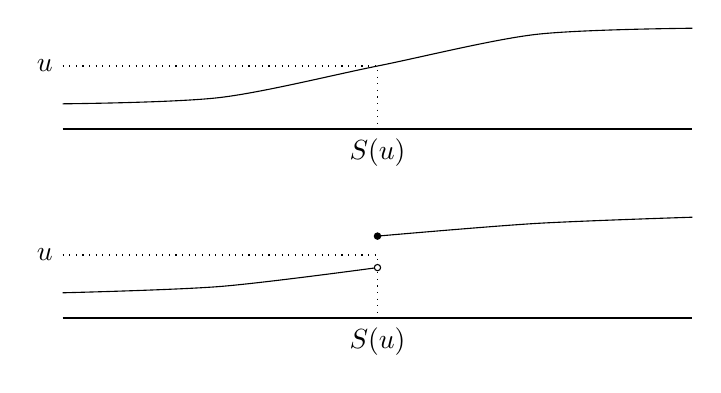
\begin{tikzpicture}[scale=.8]
      \draw (0,1) -- (10,1);
      \draw (0,4) -- (10,4); % second line
      \draw plot [smooth,tension=.5] coordinates{(0, 4.4) (2.5, 4.5) (5,5) (7.5, 5.5) (10, 5.6)};
      \draw plot [smooth,tension=.5] coordinates{(0, 1.4) (2.5, 1.5) (5,1.8)};
      \draw plot [smooth,tension=.5] coordinates{(5, 2.3) (7.5, 2.5) (10,2.6)};
      \draw[dotted] (0,5) -- (5,5) -- (5,4);
      \draw[dotted] (0,2) -- (5,2) -- (5,1);
      \draw [fill,color=white] (5,1.8) circle [radius=0.05];
      \draw (5,1.8) circle [radius=0.05];
      \draw [fill] (5,2.3) circle [radius=0.05];
      \node at (0,5) [left]{$u$};
      \node at (0,2) [left]{$u$};
      \node at (5,1) [below]{$S(u)$};
      \node at (5,4) [below]{$S(u)$};
    \end{tikzpicture}
    \caption{\small Ilustração da definição de $S(u)$.}
    \label{f:Rk_good}
  \end{figure}

  Seja $P = S_* U_{[0,1]}$, isto é $P(A) = U_{[0,1]}(S^{-1}(A))$ e mostraremos que $F_P = F$.
  Para tanto, basta ver que
  \begin{equation}
    \label{e:pseudo_inversa}
    \{u \in [0,1] \, : \,  S(u) \leq x\} = \{u \in [0,1] \, : \,  u \leq F(x)\}, \text{ para todo $x \in \mathbb{R}$}.
  \end{equation}
  Pois isso implicaria que $F_P(x) = U_{[0,1]}[S(u) \leq x] = U_{[0,1]} [u \leq F(x)] = F(x)$.

  Vamos agora checar \eqref{e:pseudo_inversa} observando que:
  \begin{enumerate}[\quad a)]
  \item Se $u \leq F(x)$ então todo $x'$ tal que $F(x') < u$ é menor que $x$.
    Logo $S(u) \leq x$.
  \item Por outro lado, se $x \ge S(u)$ então tudo $x' > x$ satisfaz $F(x') > u$. Pois por continuidade a direita $F(x)\ge u$.
  \end{enumerate}
  Isso prova \eqref{e:pseudo_inversa}, terminando a prova da proposição.
\end{proof}

\begin{exercise}
  Mostre o resultado acima usando o Teorema de Extensão de Caratheodory.
\end{exercise}


Dados espaços $\Omega_1, \dots, \Omega_n$ com suas respectivas $\sigma$-álgebras $\mathcal{F}_1, \dots, \mathcal{F}_n$, podemos definir o espaço mensurável produto $(\widebar{\Omega}, \widebar{\mathcal{F}})$ da seguinte forma
\begin{equation}
  \widebar{\Omega} = \prod_{i=1}^n \Omega_i \quad \text{e} \quad \widebar{\mathcal{F}} = \sigma \Big( \{
  A_1 \times \cdots \times A_n  \, : \,  \forall i \in \{1,\dots,n\},\ A_i \in \mathcal{F}_i \} \Big).
\end{equation}
Essa $\sigma$-álgebra é chamada de $\sigma$-álgebra produto e denotaremos ela por $\bigotimes_{i=1}^n \mathcal{F}_i$,
ou $\mathcal{F}_1\otimes \mathcal{F}_2$ quando $n=2$.

\begin{proposition}
  Se $(\Omega_1, \mathcal{F}_1, P_1), \dots, (\Omega_n, \mathcal{F}_n, P_n)$ são espaços de probabilidade, então existe uma única probabilidade $\widebar{P}$ no espaço mensurável $(\widebar{\Omega}, \widebar{\mathcal{F}})$ tal que
  \begin{equation}
    \widebar{P}(A_1 \times \cdots \times A_n) = \prod_{i=1}^n P_i(A_i), \text{ para todos $A_i \in \mathcal{F}_i$, $i \leq n$.}
  \end{equation}
  Essa probabilidade é chamada probabilidade produto.
  Usaremos a notação $\bigotimes_{i=1}^n P_i$ o $P_1\otimes P_2 \otimes \dots \otimes P_n$.
\end{proposition}

\begin{proof}
  Teoria da Medida.
\end{proof}

Note que a unicidade do produto pode ser concluída por exemplo usando o Corolário~\ref{c:produto_e_unico}.

\begin{exercise}
  Mostre que o produto de $n$ cópias de $(\{0,1\}, \mathcal{P}(\{0,1\}), \Ber(1/2))$ é a distribuição uniforme em $\{0,1\}^n$.
\end{exercise}


\subsection{Definição e propriedade básicas da esperança}

Uma noção central relacionada a distribuições em $\bbR$ e a de esperança.

\begin{definition}
  Se $X$ é uma variável aleatória com $\int_\Omega |X| P(\d \omega) < \infty$, dizemos que $X$ é integrável \index{variavel aleatoria@variável aleatória!integravel@integrável} e definimos
  \begin{equation}
    E(X) = \int_\Omega X(\omega) P(\d \omega),
  \end{equation}
\end{definition}

Quando $X \geq 0$, também podemos supor que $E(X)$ está bem definida, mesmo que possivelmente tomando valor infinito.
Não demonstraremos algumas propriedades conhecidas de medida e integração que lembramos aqui.

\begin{proposition}
 A esperança tem as seguintes propriedades:


\begin{enumerate}[\quad a)]
\item Linearidade: para qualquer $\alpha\in \bbR$, $X$ e $Y$ variável aleatórias temos (se estiverem bem definidas),
$$E(X + \alpha Y) = E(X) + \alpha E(Y)$$
\item (Teorema de convergência dominada) se $(X_n)_{n\ge 1}$ for uma sequencia de variáveis  aleatórias  tal que para todo $\go$
$|X_n(\go)|\le Z(\go)$ onde $Z(\go)$ e integrável, e tal que $\lim_{n\to \infty} X_n(\go)=X(\go)$.
Então $X$ e integrável e
$$\lim_{n\to \infty} E[X_n]=E[X].$$
 \item (Troca soma/esperança)Se $(X_n)_{n\ge 1}$ e uma família de variáveis aleatórias  tal que $\sum_{n\ge 1} E[|X_n|]<\infty$,
 então $Z:=\sum_{n\ge 1} E[X_n]$ e integrável
\item (Lema de Fatou)  se $(X_n)_{n\ge 1}$ for uma sequencia de variáveis  aleatórias  integráveis positivas ($\ge 0$), temos
$$E[\liminf X_n]\le \liminf E[X_n].$$
\item (Convergência Monótona)   se $(X_n)_{n\ge 1}$ for uma sequencia de variáveis  aleatórias  integráveis tal que
para quase todos $\go$ a sequencia $(X_n(\go))_{n\ge 0}$ então  $X=\lim_{n\to \infty} X_n(\go)$, e integrável se $E[X]$ converge
e
$$\lim_{n\to \infty} E[X_n]=E[X].$$
\item (Desigualdade de H\"older) Se $X$ e $Y$ fossem tal que $|X|^p$ e $|Y|^q$ são integráveis com $p,q>0$ tais que $p^{-1}+q^{-1}=1$
então $XY$  e integrável e
$$E[XY]\le E[|X|^p]^{1/p} E[|X|^q]^{1/q}$$

\end{enumerate}
\end{proposition}

\begin{remark}
 Se $X$ e uma variável tal que $E[|X|^p]<\infty$, para $p\in (1,\infty)$ falamos que $X\in \cL^p(P)$. \\
Observamos que o conjunto $\cL^2(P)$ tem uma estrutura natural de espaço de Hilbert
(após da operação de ter reduzido as classes de equivalência de variáveis iguais quase certamente) com produto escalar definido por
$$\langle X | Y \rangle= E[XY].$$
\end{remark}




\begin{exercise}
  Mostre que se $X \in \mathcal{L}^1$ e $P[X > x] = 0$, então $E(X) \leq x$.
\end{exercise}

\begin{lemma}
  A esperança de uma variável aleatória $X \in \mathcal{L}^1$ depende somente de sua distribuição.
  Mais precisamente
  \begin{equation}
    E(X) = \int x \; P_X (\d x).
  \end{equation}
\end{lemma}

\begin{proof}
  Vamos mostrar que
  \begin{equation}
    E\big(f(X)\big) = \int f(x) P_X (\d x),
  \end{equation}
  para toda $f: \mathbb{R} \to \mathbb{R}$ mensurável tal que $f(X) \in \mathcal{L}^1$.

  Para $f = \1_A$, temos
  \begin{equation}
    E\big(f(X)\big) = P[X \in A] =  P_X (A),
  \end{equation}
  por definição de $P_X$.

  Agora podemos extender o teorema para funções $f$ simples por linearidade,
  depois para funções positivas usando o Teorema da Convergência Monótona e
  finalmente escrevemos $x = x \1_{[0, \infty)} - (-x) \1_{(-\infty,0)}$.
\end{proof}

Vamos mostrar uma fórmula bastante simples de integração de variáveis tomando valores em um conjunto enumerável.
Se $X \in \{x_i\}_{i\in I}$ ( $I$ finito o enumerável) $P$-quase certamente, então
\begin{equation}
  \begin{split}
    E(X) & = \int_\Omega X P(\d \omega) = \int_{\Omega} \sum_{i\in I} \1_{[X = x_i]} X P(\d \omega) +
    \int_{\gO} X \1_{[X\in\bbR \setminus \{x_i\}_{i\in I}]}  P(\d \omega)\\
    & = \sum_{i\in I} \int_{[X = x_i]} x_i P(\d \omega) + 0 = \sum_{i\in I} x_i P[X = x_i].
  \end{split}
\end{equation}

Para nos acostumar à notação de probabilidade, vamos agora mostrar o mesmo resultado da seguinte forma
\begin{equation}
  \begin{split}
    E(X) & = E\Big(\sum_{i\in I} X \1_{[X = x_i]}\Big) + E(X \1_{\bbR \setminus \{x_i\}_{i\in I}})\\
    & = \sum_i E[X\, ; \, X = x_i] + 0 = \sum_{i\in I} x_i P[X = x_i],
  \end{split}
\end{equation}
que é certamente muito útil quando nos habituamos a ela.

Observe que acima usamos a notação $E[X; \mathcal{Q}] = E(X \1_{[\mathcal{Q}]})$.
Também utilizaremos $E[X; \mathcal{Q}_1, \mathcal{Q}_2, \dots] = E(X \1_{[\mathcal{Q}_1, \mathcal{Q}_2, \dots]})$

\begin{example}
  Se $X \overset{d}\sim \Ber(p)$, então $E(X) = 0 \cdot P[X = 0] + 1 P[X = 1] = 0 + p = p$.
\end{example}

\begin{example}
  Seja $X \overset{d}\sim \Bin(n,p)$,
  \begin{multline}
    E(X) = \sum_{k=0}^n\binom{n}{k}   k p^k(1-p)^{n-k}= p\partial_x \left[\sum_{k=0}^n\binom{n}{k}  x^k(1-p)^{n-k} \right]_{x=p}
    \\= p \partial_x \left[ (1-p+x)^n \right]_{x=p}=pn.
  \end{multline}
\end{example}

\begin{example}
Se $P_X(\d x) = \rho(x) \d x$ (com $\rho \geq 0$ e $\int \rho(x) \d x = 1$), então
\begin{equation}
  E(X) = \int x  P_X(\d x) = \int x \rho(x) \d x.
\end{equation}
\end{example}

\begin{example}
  Se $X \overset{d}\sim U_{[0,1]}$, então sua densidade com respeito a Lebesgue é dada por
  $P_X(\d x) = \1_{[0,1]} \d x$, donde $E(X) = \int_0^1 x \d x = 1/2$.
\end{example}

\begin{proposition}
  \label{p:espera_acumulada}
  Se $X \geq 0$ $P$-q.c., então
  \begin{equation}
    E(X) = \int_0^\infty P[X > x] \d x = \int_0^\infty [1 - F(x)] \d x .
  \end{equation}
  Se $g$ e diferenciável e tal que $E[|g'(X)|]<\infty$ então
    \begin{equation}
    E[f(X)] = \int_\bbR g'(x) [1 - F(x)] \d x .
  \end{equation}
\end{proposition}

\begin{proof}
  \begin{equation}
    \begin{split}
      E(X) & = E \Big( \int_0^X 1 \d x \Big) = E \Big( \int_0^\infty \1_{[x < X]} \d x \Big)\\
      & \overset{\text{Fubini}}= \int_0^\infty E(\1_{[x < X]}) \d x = \int_0^\infty P[x < X] \d x.
    \end{split}
  \end{equation}
    \begin{equation}
    \begin{split}
      E[f(X)] & = - E \Big( \int_{-\infty}^X f'(t)  \dd t \Big) = E \Big( \int_\bbR f'(t) \1_{[X>t]} \d x \Big)\\
      & \overset{\text{Fubini}}= \int_\bbR f'(t) E(\1_{[X>t]}) \d t = \int_\bbR f'(t) P[X>t] \d t.
    \end{split}
  \end{equation}
\end{proof}

\begin{example}
  Se $X \overset{d}\sim \Exp(\lambda)$, então
  \begin{equation}
    P[X \geq x] = \int_x^\infty \lambda e^{-\lambda t} \d t = e^{-\lambda x},
  \end{equation}
  donde
  \begin{equation}
    E(X) = \int_0^\infty e^{-\lambda x} \d x = \frac{1}{\lambda}.
  \end{equation}
\end{example}





\begin{exercise}
  Se $X \in \mathcal{L}^1$ e $P[X \geq x] = P[X \leq -x]$ para todo $x \geq 0$, então $E(X) = 0$.
\end{exercise}

% \begin{exercise}
%   Mostre que se a distribuição de $X$ tem densidade $\rho$ com respeito a Lebesgue e que $E(|f(X)|) < \infty$, então
%   \begin{equation}
%     E(f(X)) = \int f(x) \rho(x) \d x.
%   \end{equation}
% \end{exercise}

Finalmente vamos acabar essa secção estudando variáveis  do tipo $\varphi(X)$ onde $X$ e uma variável o um vector aleatório.

\begin{proposition}[Desigualdade de Jensen]
 Seja $\varphi:\bbR \to \bbR$ uma função convexa e $X$ uma variável  aleatória tal que $X$ e $\varphi(X)$ são integráveis.
 Temos
 \begin{equation}
  E[ \varphi(X) ] \le \varphi(E[X]).
 \end{equation}
 Do mesmo jeito, se $\varphi:\bbR \to \bbR^d$ e convexa e ${\bf X}$ e um vector aleatório, sob hipóteses adequadas de integrabilidade temos
  \begin{equation}
  E[ \varphi({\bf X}) ] \le \varphi(E[{\bf X}]).
 \end{equation}
\end{proposition}

\begin{remark}
  No caso onde $P_X$ tem suporte em $\{a,b\}$ o resultado e simplesmente a definição da convexidade.
  No caso $\varphi(x)=|x|^p$, $p>1$, o resultado pode ser considerado e uma consequência imediata da desigualdade de H\"older.
  No caso $\varphi(x)=|x|$, o resultado da a desigualdade triangular generalizada (que e valida para integrais com respeito a medidas positivas).
\end{remark}

\subsection{Desigualdade de Markov}

Um objectivo de muitos problemas na probabilidade e de dar cotas para probabilidade de certos eventos.
Usando a noção e esperança, obtemos um jeito muito simples de obter tais cotas.

\begin{theorem}
  \label{t:markov}
  \index{Desigualdade de Markov}
  Se $X \geq 0$ $P$-q.c., então para todo $x > 0$,
  \begin{equation}
    P[X \geq x] \leq \frac{E(X)}{x}.
  \end{equation}
\end{theorem}

\begin{proof}
  Sabemos que $X \geq x \1_{[X \geq x]}$, logo
  \begin{equation}
    E(X) \geq x E(\1_{[X \geq x]}) = x P[X \geq x],
  \end{equation}
\end{proof}



Definimos $m=E[X]$.
Sabemos por convexidade que
$$\varphi(X)\ge \varphi(m)+ a(X-m),$$
para qualquer $a\in [\varphi'_-(m), \varphi'_+(m)]$ (as derivas a esquerda e direita de $\phi$).
O resultado segue considerando a esperança nos dois lados.
(O caso vectorial fica de exercício)

\begin{topics}

\section{Tópico: Urna de Pólya}
\label{s:urna_polya}

Um excelente exemplo de como Cadeias de Markov podem gerar interessantes modelos de situações reais são as chamadas Urnas de Pólya.
Esse processo modela sistemas de física, biologia, computação e economia que apresentam o que chamamos de reforço.

Tome por exemplo duas empresas que competem pelo mercado de aviões.
Inicialmente, não temos nenhuma razão para escolher uma em detrimento da outra, portanto compramos nosso primeiro avião de cada empresa com probabilidade meio.
Porém, depois que já compramos diversos aviões de uma determinada empresa, ela já recebeu bastante dinheiro que pode ser reinvestido para gerar melhor tecnologia e aumentar as chances que ela seja escolhida novamente no futuro.
Isso é o que chamamos de reforço.

Vamos agora apresentar rigorosamente um modelo para situações desse tipo.
O nosso modelo começa com uma urna contendo duas bolas, uma vermelha e uma azul.
No cada passo do processo, escolheremos uma bola da urna ao acaso, olharemos sua cor e retornaremos essa bola para dentro urna junto com mais uma bola da mesma cor.
Isso pode será formalizado à seguir.

Vamos construir uma medida em $\{0, 1\}^\mathbb{N}$, dotado da $\sigma$-álgebra produto.
Fixada uma sequência finita $w_1, \dots, w_n$ em $\{0,1\}$, definimos
\begin{equation}
  N_x (w_1, \dots, w_n) = \# \big\{ j \in \{1, \dots, n\}\, : \, w_j = x \big\} + 1,
\end{equation}
que nada mais é que o número de bolas do tipo $x$ que se encontram na urna no tempo $n$.
Quando tivermos uma sequência infinita de $w_i$'s, escreveremos $N^n_x$ para denotar $N_x(w_1, \dots, w_n)$.

Para cada $n \geq 1$, definimos $K_n:\{0,1\}^n \to \mathcal{P}(\{0,1\})$ por
\begin{equation}
  K_n(w_1, \dots, w_n) = \Ber\big( \tfrac{N_1}{n} \big).
\end{equation}
Ou seja, dadas cores $w_1, \dots, w_n$, escolheremos uma bola de cor $1$ proporcionalmente ao número $N_1$ de bolas de cor $1$ que já foram sorteadas.

\begin{exercise}
  \label{x:constr_Polya}
  Mostre que todos $K_n$ acima definem núcleos de transição.
  Além disso a seguinte sequência de medidas é compatível no sentido de Kolmogorov:
  \begin{itemize}
  \item $P_1 = \Ber(1/2)$,
  \item $P_2 = P_1 \star K_1$,
  \item $P_3 = P_2 \star K_2, \dots$
  \end{itemize}
  Conclua que existe a medida $P$ em $\{0,1\}^\mathbb{N}$ que define o modelo de Pólya.
\end{exercise}

Podemos agora fazer perguntas como por exemplo: será que escolheremos bolas de ambas as cores para sempre, ou a partir de um certo momento escolheremos bolas de apenas uma cor com certa probabilidade.
Mais precisamente, qual é a probabilidade de $[X_i = 1, \text{ infinitas vezes}]$?


Para responder perguntas desse tipo, iremos mostrar algo muito curioso, que pode ser entendido como uma outra maneira de representar o modelo descrito acima.
Mas antes, vamos colecionar alguns fatos sobre o modelo da Urna de Pólya.

Primeiramente vamos olhar para os seguintes eventos.
Fixamos $n \geq 1$ e uma sequência $w_1, \dots, w_n \in \{0,1\}$ e seja $A$ o evento $\{w_1\} \times \dots \times \{w_n\} \times \{0,1\} \times \dots$
Note que os eventos desse tipo (junto com o evento $\varnothing$) formam um $\pi$-sistema que gera a $\sigma$-álgebra canônica de $\{0,1\}^\mathbb{N}$, portanto essa coleção é bastante completa para identificar a distribuição da Urna de Pólya.

Podemos calcular a probabilidade do evento $A$ acima
\begin{equation}
  \begin{split}
    P(A) & = \frac{N^1_{w_1}}2 \frac{N^2_{w_1}}3 \dots \frac{N^n_{w_n}}{n+1} = \frac{1}{(n+1)!} \prod_{i=1}^n N^i_{w_i}\\
    & = \frac{N^n_1! (n - N^n_1)!}{(n+1)!} = \frac{1}{(n+1)} \binom{n}{N^n_1}^{-1}.
  \end{split}
\end{equation}
O que é muito interessante sobre a equação acima é que ela nos remete a problemas combinatórios ao notarmos o fator binomial acima.

Vamos portanto construir um processo completamente diferente que apresenta as mesmas probabilidades que o anterior.
Seja $\mathcal{S}_N$ o conjunto de todas as permutações $\sigma$ de $\{1,\dots,N\}$.
É fácil ver que
\begin{equation*}
  \frac{1}{(n+1)} \binom{n}{j}^{-1} = U_{\mathcal{S}_{n+1}} \Big[ \sigma(n+1) =j+1, \sigma(i) \leq j \text{ se e só se } \; i \leq j \Big].
\end{equation*}

Um método muito interessante de se produzir uma permutação uniforme é dado pelos seguintes exercícios.

\begin{exercise}
  Seja $n \geq 1$ um inteiro, $P$ uma probabilidade em $(E, \mathcal{A})$, $\sigma$ uma permutação fixa em $\mathcal{S}_n$.
  Então
  \begin{equation}
    \label{e:intercambiavel}
    (X_1, \dots, X_n) \distr (X_{\sigma(1)}, \dots, X_{\sigma(n)}),
  \end{equation}
  onde $X_i$ como sempre representam as coordenadas canônicas em $(E^{n}, \mathcal{A}^{\otimes n}, P^{\otimes n})$.
\end{exercise}

Ou em outras palavras, aplicar uma permutação fixa a uma sequência \iid não altera sua distribuição.
Sequências de elementos aleatórios (não necessariamente \iid's) que satisfazem \eqref{e:intercambiavel} são ditas intercambiáveis. \index{sequencias@sequências!intercambiaveis@intercambiáveis}

Um outro exercício interessante nesse tópico é o seguinte
\begin{exercise}
  Seja $n \geq 1$ e $F:[0,1]^n \to \mathcal{S}_n$ dada por
  \begin{equation*}
    F(x_1, \dots, x_n) =
    \begin{cases}
      (1, 2, \dots, n), \qquad \text{se existe $i \neq j$ com $x_i = x_j$, }\\
      \text{o único $\sigma$ tal que $x_{\sigma(1)} < \dots < x_{\sigma(n)}$,} \qquad \text{caso contrário.}
    \end{cases}
  \end{equation*}
  Mostre que $F_*(U_{[0,1]}^{\otimes n}) = U_{\mathcal{S}_n}$.
\end{exercise}

Ou seja, ordenar uma sequência de uniformes independentes nos fornece uma permutação uniforme.
Como prometido, isso nos dá uma maneira de construir uma permutação uniforme de $\{1, \dots, n\}$ à partir de uma sequência \iid (que é algo que já estamos começando a entender melhor).

Podemos agora escrever nossa probabilidade de observar uma sequência no modelo da Urna de Pólya em termos de uma sequência \iid de variáveis aleatórias.
\begin{equation*}
  \begin{split}
    \frac{1}{(n+1)} & \binom{n}{N^n_1}^{\mathclap{\;-1}} =
    F_{*} U_{[0,1]}^{\otimes n+1} \Big[ \sigma(n+1) = N^n_1 + 1, \sigma(i) \leq N^n_1 \text{ se e só se } i \leq N^n_1 \Big]\\
    & =  U^{\otimes n+1}_{[0,1]} \Big[ \text{$X_i < X_{n+1}$, para $i \leq N^n_1$ e $X_i > X_{n+1}$, para $i \ge N^n_1+1$} \Big].
  \end{split}
\end{equation*}
Agora estamos prontos para provar o resultado principal que nos ajudará a calcular probabilidades no modelo da Urna de Pólya.

Dado $u \in [0,1]$, seja $P_u = \Ber(u)^{\otimes \mathbb{N}}$, ou seja a probabilidade que nos dá uma sequência infinita de moedas independentes com probabilidade $u$ de sucesso.
Definimos agora $\widebar{K}: [0,1] \times (\mathcal{P}(\{0,1\})^{\otimes \mathbb{N}}) \to [0,1]$ dada por
\begin{equation}
  \widebar{K}(u,A) = P_u(A).
\end{equation}

\begin{lemma}
  A função $\widebar{K}$ definida acima é um núcleo entre $[0,1]$ e $\{0,1\}^{\mathbb{N}}$.
\end{lemma}

\begin{proof}
  Usando a Proposição~\ref{p:K_nucleo_na_classe}, basta ver que
  \begin{display}
    para todo $k \geq 1$ e $w_1, \dots, w_k \in \{0,1\}$, temos que $P_u(X_1 = w_1, \dots, X_k = w_k)$ é uma função mensurável de $u \in [0,1]$.
  \end{display}
  Mas é fácil ver que
  \begin{equation}
    \label{e:Polya_binomial}
    P_u(X_1 = w_1, \dots, X_k = w_k) = u^{N_1(w_1, \dots, w_k)} (1 - u)^{N_0(w_1, \dots, w_k)},
  \end{equation}
  que obviamente é mensurável, provando assim o lema.
\end{proof}

O resultado muito curioso a qual nos referimos é o seguinte.

\begin{lemma}
  A lei $P$ definida no Exercício~\ref{x:constr_Polya} é igual a $U_{[0,1]} \widebar{K}$.
\end{lemma}

Em outras palavras, digamos que realizamos os seguintes experimentos.
Primeiramente João realiza o processo da Urna de Pólya e anota a sequência das cores obtidas.
Depois Maria sorteia uma variável aleatória $X$ de distribuição uniforme em $[0,1]$ e depois joga infinitas vezes uma moeda com probabilidade $X$ de obter vermelho e $(1-X)$ de obter azul, anotando também quais cores foram obtidas.
Finalmente, não seríamos capazes de distinguir essas duas sequências (mesmo que pudéssemos repetir várias vezes esse experimento) pois elas tem a mesma distribuição em $\{0,1\}^{\mathbb{N}}$.

\begin{proof}
  Já sabemos que basta mostrar a igualdade para eventos do tipo $A = \{w_1\} \times \dots \times \{w_n\} \times \{0,1\}^\mathbb{N}$.
  Sabemos pelo Teorema de Fubini para Núcleos que
  \begin{equation}
    U_{[0,1]} \widebar{K}(A) = \int_0^1 K(u, A) \d u \overset{\eqref{e:Polya_binomial}}= \int_0^1 u^{N_1(w_1, \dots, w_k)} (1 - u)^{N_0(w_1, \dots, w_k)} \d u.
  \end{equation}

  Por outro lado , sabemos (usando simetria entre $0$ e $1$) que
  \begin{equation}
    P(A) = U^{\otimes n+1}_{[0,1]} \Big[ \text{$X_i < X_{n+1}$, para $i \leq N^n_0$ e $X_i > X_0$, para $i \ge N^n_0+1$} \Big]
  \end{equation}

  Se definirmos $\tilde{K}:[0,1] \times \mathcal{B}([0,1]^n)$, dado por $\tilde{K}(u,B) =  U^{\otimes n}_{[0,1]}$, sabemos que isso define um núcleo pelo Exercício~\ref{x:nucleo_constante}.
  Mais ainda, esse mesmo exercício nos diz que $U_{[0,1]} \star \tilde{K} =
   U^{\otimes}_{[0,1]}$, de forma que
  \begin{equation*}
    \begin{split}
      P(A) & = U_{[0,1]} \star \tilde{K} \Big[ \text{$X_i < X_0$, para $i \leq N^n_0$ e $X_i > X_0$, para $i\ge N^n_0+1$} \Big]\\
      & = \int_0^1  U^{\otimes n}_{[0,1]} \Big[ \text{$X_i < u$, para $i \leq N^n_0$ e $X_i > u$, para $i \ge N^n_0+1$} \Big] \d u\\
      & = \int_0^1 u^{N^n_0} (1-u)^{n - N^n_0} \d u,
    \end{split}
  \end{equation*}
  que coincide com $U_{[0,1]} \widebar{K}(A)$, provando o lema.
\end{proof}

\begin{exercise}
  Mostre que a probabilidade, segundo o modelo da Urna de Pólya, de que observemos infinitas bolas de ambas as cores é um.
\end{exercise}

\end{topics}



%%% Local Variables:
%%% mode: latex
%%% TeX-master: "../Notas_de_aula"
%%% End:
